
\providecommand{\Fun}{\operatorname{Fun}}
\providecommand{\QCat}{\mathcal{Q}\mathcal{C}at}
\providecommand{\sSet}{s\mathcal{S}et}
\providecommand{\Kan}{\mathcal{K}an}
\providecommand{\coreS}{\mathrm{core}_{\ast}}   %
\providecommand{\Disc}{\mathcal{D}\mathrm{isc}} %

\section{反\texorpdfstring{$(\infty,1)$}{(∞,1)}-范畴与∞-群胚核}%
\label{sec:opposite-infinity-1-categories-and-infinity-groupoid-cores}

第 1 章中的\cref{def:co-dual-cosmoi}对一个\trInfinityCosmos{}之余对偶所作的
构造，用到了单纯集之反者的构造。请回忆：单纯集
$X\colon\boldsymbol{\Delta}^{\mathrm{op}}\to\mathcal{S}et$ 的反者，是经由与
对象上恒等的对合 $(-)^{\circ}\colon\boldsymbol{\Delta}\to\boldsymbol{\Delta}$
——它反转每个序数 $[n]\in\boldsymbol{\Delta}$ 中元素的排序——作\trPreComposition{}而
得到。与 $(-)^{\circ}$ 作\trPreComposition{}定义了一个\trFunctor{}
$(-)^{\mathrm{op}}\colon\sSet\to\sSet$，它把一个\trSimplicialSet{} $X$ 送到
其\textbf{\trOppositeSimplicialSet} $X^{\mathrm{op}}$。我们首先探究这一运算
在\trQuasiCategory{}的\trInfinityCosmos{}中所扮演的角色，随后再于其他
∞-\trCategory{}的\trInfinityCosmos{}中考察一个相关的运算。

\begin{lemma}\label{lem:opposite-quasi-category}
若 $X$ 是一个\trQuasiCategory，则 $X^{\mathrm{op}}$ 是一个\trQuasiCategory。
\end{lemma}

\begin{proof}
下方左侧的\trLifting{}问题由下方右侧的\trLifting{}问题求解：
\begin{center}
\begin{tikzpicture}[x=1.5em,y=1.5em]
  \node (a1) at (0,1.3) {$\Lambda^{k}[n]$};
  \node (b1) at (3.0,1.3) {$X^{\mathrm{op}}$};
  \node (c1) at (0,0)   {$\Delta[n]$};
  \draw[->] (a1) -- (b1);
  \draw[right hook->] (0,0.95) -- (0,0.3);
  \draw[->,dashed] (0.45,0.2) -- (2.6,1.1);
  \node at (4.9,0.65) {$\leftrightsquigarrow$};
  \node (a2) at (6.8,1.3) {$\Lambda^{n-k}[n]$};
  \node (b2) at (9.8,1.3) {$X$};
  \node (c2) at (6.8,0)   {$\Delta[n]$};
  \draw[->] (a2) -- (b2);
  \draw[right hook->] (6.8,0.95) -- (6.8,0.3);
  \draw[->,dashed] (7.25,0.2) -- (9.4,1.1);
\end{tikzpicture}
\end{center}
\end{proof}

\begin{definition}\label{def:opposite-quasi-category}
对一个\trQuasiCategory{} $A$，其\textbf{反拟范畴}（opposite quasi-category）
$A^{\mathrm{op}}$ 是由「反转每个单纯形中诸顶点的排序」所定义的单纯集。
\end{definition}

\begin{lemma}\label{lem:opposite-qcat-biequivalence}
反拟范畴构造定义了一个对合的\trCosmologicalBiequivalence{}
$(-)^{\mathrm{op}}\colon\QCat\rightsquigarrow\QCat^{\mathrm{co}}$，其在%
\trFunctorSpace{}上的作用经由一个自然\trIsomorphism
\[
\Fun(A,B)\xrightarrow{\ \sim\ }\Fun(A^{\mathrm{op}},B^{\mathrm{op}})^{\mathrm{op}}.
\]
给出。
\end{lemma}

\begin{proof}
\trIsomorphism{} $\Fun(A,B)\cong\Fun(A^{\mathrm{op}},B^{\mathrm{op}})^{\mathrm{op}}$
最好在单纯形的层面上来理解：定义\trFunctorSpace{} $\Fun(A,B)$ 中诸 $n$-单纯形
的那些单纯映射 $A\times\Delta[n]\to B$，经由\trIsomorphism{}
$(-)^{\mathrm{op}}\colon\sSet\simeq\sSet$ 被送到单纯映射
$A^{\mathrm{op}}\times\Delta[n]^{\mathrm{op}}\to B^{\mathrm{op}}$，而这些映射
定义了\trFunctorSpace{} $\Fun(A^{\mathrm{op}},B^{\mathrm{op}})^{\mathrm{op}}$
中的诸 $n$-单纯形。

由\cref{lem:opposite-quasi-category}之证明的一个扩张，一个\trIsofibration{}的反者仍是一个%
\trIsofibration。$\QCat$ 中的诸\trCone{}形\trLimit{}由于在 $\mathcal{S}et$ 中
逐点定义，故沿\trFunctor{} $(-)^{\circ}\colon\boldsymbol{\Delta}\to\boldsymbol{\Delta}$
的限制而得到保持。单纯\trCotensor{}亦得到保持：对一个\trQuasiCategory{} $B$
与一个\trSimplicialSet{} $X$，有
$(B^{X})^{\mathrm{op}}\cong(B^{\mathrm{op}})^{X^{\mathrm{op}}}$，这与第 1 章
中的\cref{def:co-dual-cosmoi}所指出的、$\QCat^{\mathrm{co}}$ 中的
$B^{\mathrm{op}}$ 与\trSimplicialSet{} $X$ 之\trCotensor{}的一般构造相合。这
就证明了 $(-)^{\mathrm{op}}\colon\QCat\to\QCat^{\mathrm{co}}$ 定义一个%
\trCosmologicalFunctor。
\end{proof}

\cref{lem:opposite-qcat-biequivalence}扩张了 1-\trCategory{}之反者的通常构造
以及相应的 2-\trFunctor{}
$(-)^{\mathrm{op}}\colon\mathcal{C}at\to\mathcal{C}at^{\mathrm{co}}$（见练习
B.2.iii）。%
由于\cref{def:opposite-quasi-category}所给的构造是显式的，一个\trQuasiCategory{}的反者是在%
\trIsomorphism{}意义下定义的。相比之下，在不附加任何假设时，对一个双等价的%
\trInfinityCosmos{}中的\trInfinityCategory，我们只能把其反者定义到%
\trEquivalence{}为止。\footnote{在我们所知的每一个 $(\infty,1)$-%
\trCategory{}的模型中，事实上都存在一个严格定义的 op-对合，而且可以验证：
这些以解析方式定义的反∞-\trCategory{}与标准的\trChangeOfModel{}\trFunctor{}%
相容。然而，为验证反∞-\trCategory{}构造在每一情形中的严格相容性所需付出的
力气，或许不值得这份额外严格性所带来的好处。}虽然这初看似乎不合人意，但以
这种方式给出定义可以说才是在道理上正确的，因为从模型无关的观点看，%
\trInfinityCategory{}本身也只应当被考虑到\trEquivalence{}为止。

\begin{definition}\label{def:opposite-infinity-category}
设 $A$ 是一个 $(\infty,1)$-\trCategory{}的\trInfinityCosmos{} $\mathcal{K}$
中的一个\trInfinityCategory。定义其\textbf{反∞-\trCategory}（opposite
∞-category）$A^{\mathrm{op}}$ 为 $\mathcal{K}$ 中任何一个其底\trQuasiCategory{}%
为 $A_{0}^{\mathrm{op}}$ 的\trInfinityCategory。
\end{definition}

我们现在论证：\cref{def:opposite-infinity-category}在\trEquivalence{}意义下
是良定义的：

\begin{proposition}\label{prop:opposite-quasi-pseudofunctor}
在一个 $(\infty,1)$-\trCategory{}的\trInfinityCosmos{} $\mathcal{K}$ 中，
任何一组对反∞-\trCategory{}的选取都装配成一个拟伪\trFunctor{}与%
\trBiequivalence{} $(-)^{\mathrm{op}}\colon\mathcal{K}\rightsquigarrow\mathcal{K}^{\mathrm{co}}$。
特别地，对任意\trInfinityCategory{} $A,B\in\mathcal{K}$，存在一个%
\trEquivalence{} $\Fun(A,B)\simeq\Fun(A^{\mathrm{op}},B^{\mathrm{op}})^{\mathrm{op}}$，
它在 $A$ 与 $B$ 上都是拟伪自然的。
\end{proposition}

\begin{proof}
这一拟伪\trFunctor{}性的\trBiequivalence{}定义为诸\trCosmologicalBiequivalence{}%
的之字形链之复合
\begin{center}
\begin{tikzpicture}[x=1.8em,y=1.5em]
  \node (tl) at (0,1.6) {$\mathcal{K}$};
  \node (tr) at (5.6,1.6) {$\mathcal{K}^{\mathrm{co}}$};
  \draw[->] (0.9,1.6) -- ++(0.54,0.07) -- ++(0.55,-0.14) -- ++(0.54,0.14)
    -- ++(0.55,-0.14) -- ++(0.54,0.14) -- ++(0.55,-0.14) -- ++(0.54,0.07);
  \node at (2.8,2.0) {$\scriptstyle(-)^{\mathrm{op}}$};
  \draw[right hook->] (0,1.1) -- (0,0.45);
  \node at (-0.85,0.78) {$\scriptstyle(-)_{0}$};
  \node at (2.8,0.78) {$\scriptstyle\cong$};
  \draw[right hook->] (5.6,1.1) -- (5.6,0.45);
  \node at (6.45,0.78) {$\scriptstyle(-)_{0}$};
  \node (bl) at (0,0) {$\QCat$};
  \node (br) at (5.6,0) {$\QCat^{\mathrm{co}}$};
  \draw[->] (0.9,0) -- node[above]{$\scriptstyle\sim$}
    node[below]{$\scriptstyle(-)^{\mathrm{op}}$} (4.7,0);
\end{tikzpicture}
\end{center}
我们首先为每个 $A\in\mathcal{K}$ 选取反∞-\trCategory，连同指定的伴随%
\trEquivalence{} $(A^{\mathrm{op}})_{0}\simeq(A_{0})^{\mathrm{op}}$。与这些%
\trEquivalence{}作复合后，\trBiequivalence{} $(-)_{0}\colon\mathcal{K}\to\QCat$
提供诸\trQuasiCategory{}之间的局部\trEquivalence：
\begin{center}
\begin{tikzpicture}[x=1.5em,y=1.5em]
  \node (tl) at (0,1.6) {$\Fun(A,B)$};
  \node (tr) at (8.4,1.6) {$\Fun(A^{\mathrm{op}},B^{\mathrm{op}})^{\mathrm{op}}$};
  \draw[->,dashed] (tl) -- node[above]{$\scriptstyle\sim$} (tr);
  \draw[right hook->] (0,1.15) -- (0,0.45);
  \draw[right hook->] (8.4,1.15) -- (8.4,0.45);
  \node at (4.6,0.8) {$\scriptstyle\cong$};
  \node (bl) at (0,0) {$\Fun(A_{0},B_{0})$};
  \node[anchor=west] (br) at (2.5,0)
    {$\xrightarrow{\ \sim\ }\Fun((A_{0})^{\mathrm{op}},(B_{0})^{\mathrm{op}})^{\mathrm{op}}\cong\Fun((A^{\mathrm{op}})_{0},(B^{\mathrm{op}})_{0})^{\mathrm{op}}$};
\end{tikzpicture}
\end{center}
它们复合而定义所需的\trEquivalence，且使得该方块在一个同伦相干\trIsomorphism{}%
之下交换。为使这些\trEquivalence{}定义一个拟伪\trFunctor{}在诸%
\trFunctorSpace{}上的作用，我们遵循推论 10.4.17 的构造——如其于命题 10.4.16
之证明中所描述者——选取左下方那个水平单纯自然\trEquivalence{}的伴随%
\trEquivalence{}逆，并应用引理 10.4.15。引理 10.4.12 随即证明该拟伪自然性
陈述。
\end{proof}

鉴于\trEquivalence{}
$\Fun(A,B)\simeq\Fun(A^{\mathrm{op}},B^{\mathrm{op}})^{\mathrm{op}}$，
$(\infty,1)$-\trCategory{}之间的一个\trFunctor{} $f\colon A\to B$ 拥有一个
反\trFunctor{} $f^{\mathrm{op}}\colon A^{\mathrm{op}}\to B^{\mathrm{op}}$；
一旦定义域与余域的\trInfinityCategory{}已被固定，它便在\trIsomorphism{}意义
下良定义。类似地，平行\trFunctor{}之间的一个\trNaturalTransformation{}拥有
一个反者
\begin{center}
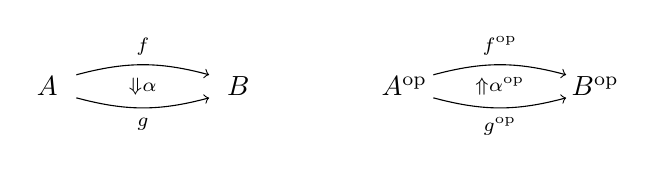
\begin{tikzpicture}[x=1.5em,y=1.3em]
  \node (A) at (0,0) {$A$};
  \node (B) at (4.6,0) {$B$};
  \draw[->] (0.7,0.32) to[bend left=15] node[above,pos=0.5]{$\scriptstyle f$} (3.9,0.32);
  \draw[->] (0.7,-0.32) to[bend right=15] node[below,pos=0.5]{$\scriptstyle g$} (3.9,-0.32);
  \node at (2.3,0) {$\scriptstyle\Downarrow\alpha$};
  \node at (6.6,0) {$\scriptstyle\leftrightsquigarrow$};
  \begin{scope}[shift={(8.6,0)}]
    \node (Ao) at (0,0) {$A^{\mathrm{op}}$};
    \node (Bo) at (4.6,0) {$B^{\mathrm{op}}$};
    \draw[->] (0.7,0.32) to[bend left=15] node[above,pos=0.5]{$\scriptstyle f^{\mathrm{op}}$} (3.9,0.32);
    \draw[->] (0.7,-0.32) to[bend right=15] node[below,pos=0.5]{$\scriptstyle g^{\mathrm{op}}$} (3.9,-0.32);
    \node at (2.3,0) {$\scriptstyle\Uparrow\alpha^{\mathrm{op}}$};
  \end{scope}
\end{tikzpicture}
\end{center}
它是通过施加命题 12.1.5 的拟伪\trFunctor{}所底蕴的那个伪\trFunctor{}
$(-)^{\mathrm{op}}\colon\mathfrak{h}\mathcal{K}\rightsquigarrow\mathfrak{h}\mathcal{K}^{\mathrm{op}}$
而得到的。此外：

\begin{lemma}\label{lem:op-of-cotensor-and-hom}
设 $\mathcal{K}$ 是一个 $(\infty,1)$-\trCategory{}的\trInfinityCosmos。
\begin{enumerate}[label=(\roman*)]
\item 对任何\trInfinityCategory{} $A$ 与\trSimplicialSet{} $U$，有
  $(A^{U})^{\mathrm{op}}\simeq(A^{\mathrm{op}})^{U^{\mathrm{op}}}$。
\item 对任何\trFunctor{} $f\colon B\to A$ 与 $g\colon C\to A$，存在
  $B^{\mathrm{op}}\times C^{\mathrm{op}}$ 之上的一个\trEquivalence
  $\mathrm{Hom}_{A}(f,g)^{\mathrm{op}}\simeq\mathrm{Hom}_{A^{\mathrm{op}}}(g^{\mathrm{op}},f^{\mathrm{op}})$。
\end{enumerate}
\end{lemma}

\begin{proof}
我们有一条拟伪自然的\trEquivalence：
\begin{align*}
\Fun(X,(A^{U})^{\mathrm{op}})
  &\simeq\Fun(X^{\mathrm{op}},A^{U})^{\mathrm{op}}
  &&\text{由 \cref{prop:opposite-quasi-pseudofunctor}}\\
  &\simeq(\Fun(X^{\mathrm{op}},A)^{U})^{\mathrm{op}}
  &&\text{由 \eqref{eq:cotensor-universal}}\\
  &\simeq(\Fun(X^{\mathrm{op}},A)^{\mathrm{op}})^{U^{\mathrm{op}}}
  &&\text{由 \cref{lem:opposite-qcat-biequivalence}}\\
  &\simeq\Fun(X,A^{\mathrm{op}})^{U^{\mathrm{op}}}
  &&\text{由 \cref{prop:opposite-quasi-pseudofunctor}}\\
  &\simeq\Fun(X,(A^{\mathrm{op}})^{U^{\mathrm{op}}})
  &&\text{由 \eqref{eq:cotensor-universal}}.
\end{align*}
故由引理 10.4.14，$(A^{U})^{\mathrm{op}}\simeq(A^{\mathrm{op}})^{U^{\mathrm{op}}}$。

第二个陈述是一个更一般结果的推论：任何拟伪\trFunctor{}性的\trBiequivalence
——例如命题 12.1.5 所确立的
$(-)^{\mathrm{op}}\colon\mathcal{K}\rightsquigarrow\mathcal{K}^{\mathrm{co}}$
——保持并反射诸\trCommaInfinityCategory。或者，由于此处所论的拟伪%
\trFunctor{}性的\trBiequivalence{}定义为诸\trCosmologicalBiequivalence{}的
之字形链，该结果也可由「诸\trCosmologicalBiequivalence{}本身保持并反射诸%
\trCommaInfinityCategory」这一事实——如命题 10.3.6(vi) 所观察到者——得出。
\end{proof}

下一个结果为「诉诸对偶性」提供了另一种视角：此前，关于一个\trInfinityCosmos{}
$\mathcal{K}$ 中诸\trDiagram{}之\trColimit{}的事实，是从关于
$\mathcal{K}^{\mathrm{co}}$ 中诸\trLimit{}的相应证明中演绎而得的；类似地，
关于\trCartesianFibration{}的结果也是在 $\mathcal{K}^{\mathrm{co}}$ 中得到
解读，从而得出关于 $\mathcal{K}$ 中\trCocartesianFibration{}的相应
结果。

\begin{proposition}\label{prop:duality-for-limits-and-fibrations}
设 $\mathcal{K}$ 是一个 $(\infty,1)$-\trCategory{}的\trInfinityCosmos。
\begin{enumerate}[label=(\roman*)]
\item $A$ 中一个 $J$ 形状的图表族拥有一个\trColimit，当且仅当 $A^{\mathrm{op}}$
  中相应的 $J^{\mathrm{op}}$ 形状的图表族拥有一个\trLimit。
\item 一个\trFunctor{} $p\colon E\twoheadrightarrow B$ 定义一个%
  \trCartesianFibration，当且仅当\trFunctor{}
  $p^{\mathrm{op}}\colon E^{\mathrm{op}}\twoheadrightarrow B^{\mathrm{op}}$
  定义一个\trCocartesianFibration。\footnote{正如第三部分的引言中所指出的，
  由 $p^{\mathrm{op}}$ 所编码的同伦相干\trDiagram{}并\emph{不}是由 $p$ 所
  编码的同伦相干\trDiagram{}——这是 Bénabou 的一个经典观察，经 Barwick、
  Glasman 与 Nardin 扩展到 $(\infty,1)$-范畴的语境 $[7]$。}
\end{enumerate}
\end{proposition}

注意：若 $p\colon E\twoheadrightarrow B$ 是一个\trIsofibration，那么总可能
选取一个\trFunctor{}
$p^{\mathrm{op}}\colon E^{\mathrm{op}}\twoheadrightarrow B^{\mathrm{op}}$
使其仍是一个\trIsofibration，或许需要更换全空间 $E^{\mathrm{op}}$ 的选取。

\begin{proof}
由\cref{lem:op-of-cotensor-and-hom}，$A$ 中一个 $J$ 形状的图表族
$d\colon D\to A^{J}$ 定义一个 $J^{\mathrm{op}}$ 形状的图表族
$d^{\mathrm{op}}\colon D^{\mathrm{op}}\to(A^{\mathrm{op}})^{J^{\mathrm{op}}}$。
由命题 4.3.1，%
$d$ 在 $A$ 中容有一个\trColimit，当且仅当存在诸\trCommaInfinityCategory{}的
一个\trEquivalence
\begin{equation*}
\mathrm{Hom}_{A^{J}}(d,\Delta)\simeq_{A\times D}\mathrm{Hom}_{A}(c,A),
\end{equation*}
此时，表示\trFunctor{} $c\colon D\to A$ 定义余极限\trFunctor。

由\cref{lem:op-of-cotensor-and-hom}，这样一个\trEquivalence{}存在，当且仅当
存在一个\trEquivalence
\begin{equation*}
\mathrm{Hom}_{(A^{\mathrm{op}})^{J^{\mathrm{op}}}}(\Delta,d^{\mathrm{op}})
\simeq_{D^{\mathrm{op}}\times A^{\mathrm{op}}}
\mathrm{Hom}_{A^{\mathrm{op}}}(A^{\mathrm{op}},c^{\mathrm{op}}),
\end{equation*}
而由命题 4.3.1，后者刻画了极限\trFunctor{}
$c^{\mathrm{op}}\colon D^{\mathrm{op}}\to A^{\mathrm{op}}$。

第二个陈述类似地证明。由第 5 章中的\cref{thm:internal-characterization}，
$p\colon E\twoheadrightarrow B$ 定义一个\trCartesianFibration，当且仅当受
诱导的\trFunctor{}
$i_{1}\hat{\delta}p\colon E^{2}\twoheadrightarrow\mathrm{Hom}_{B}(B,p)$
容有一个右伴随右逆。施加拟伪\trFunctor{}性的\trBiequivalence{}
$(-)^{\mathrm{op}}\colon\mathcal{K}\rightsquigarrow\mathcal{K}^{\mathrm{co}}$，
这个\trAdjunction{}存在，当且仅当那个反\trFunctor{}容有一个左伴随右逆。这个%
\trFunctor{}未必\trIsomorphism{}于
$i_{0}\hat{\delta}p^{\mathrm{op}}\colon(E^{\mathrm{op}})^{2}\twoheadrightarrow\mathrm{Hom}_{B^{\mathrm{op}}}(p^{\mathrm{op}},B^{\mathrm{op}})$，
但由\cref{lem:op-of-cotensor-and-hom}它与后者\trEquivalence{}，而由伴随的%
\trEquivalence{}不变性，这就足够了（见练习 B.4.i）。由第 5 章中的%
\cref{thm:internal-characterization}的对偶，这样一个\trAdjunction{}存在，
当且仅当 $p^{\mathrm{op}}\colon E^{\mathrm{op}}\twoheadrightarrow B^{\mathrm{op}}$
是一个\trCocartesianFibration。
\end{proof}

我们现在把注意力转向一个\trQuasiCategory{}的 Kan 复形核的构造，并讨论其在
其他 $(\infty,1)$-\trCategory{}的\trInfinityCosmos{}中的类比。

\begin{definition}\label{def:infinity-groupoid-core-quasi-category}
一个\trQuasiCategory{} $A$ 的\textbf{\trInfinityGroupoidCore}（∞-groupoid
core）是最大的\trKanComplex{} $\mathrm{core}A\subseteq A$，它可构造为包含
下列成分的单纯子集：
\begin{itemize}
\item $A$ 的全部顶点；
\item 恰那些在 $A$ 中定义\trIsomorphism{}的边（见第 1 章中的%
  \cref{def:isomorphism-quasi-category}）；
\item 每条边皆为\trIsomorphism{}的更高维单纯形。
\end{itemize}
\end{definition}

\begin{lemma}\label{lem:core-is-kan-complex}
一个\trQuasiCategory{}的\trInfinityGroupoidCore{}是一个\trKanComplex，而且
它确实是含于该\trQuasiCategory{} $A$ 之中的最大\trKanComplex。
\end{lemma}

\begin{proof}
\cref{def:infinity-groupoid-core-quasi-category}中所构造的包含 $\mathrm{core}A\subset A$ 在除维数一以外的所有
维数的单纯形上都是满的。于是，为见 $\mathrm{core}A$ 是一个\trQuasiCategory，
只需论证它沿\trHorn{} $\Lambda^{1}[2]\hookrightarrow\Delta[2]$ 容有%
\trExtension。由构造，一支\trHorn{} $\Lambda^{1}[2]\to\mathrm{core}A$ 选取出
$A$ 中的两个\trIsomorphism。填充体 $\Delta[2]\to A$ 见证\trHomotopyCategory{}
$\mathrm{h}A$ 中的一个复合关系；于是该复合边也是\trIsomorphism，且由满性，
这个填充体提升为 $\Delta[2]\to\mathrm{core}A$。

由构造，$\mathrm{h}(\mathrm{core}A)$ 是一个\trGroupoid；而且它是含于
$\mathrm{h}A$ 中的极大子\trGroupoid。于是由第 1 章中的\cref{cor:kan-groupoid}，
$\mathrm{core}A$ 是一个\trKanComplex。

最后，一个中间单纯子集 $\mathrm{core}A\subsetneq K\subset A$ 必然包含一条
额外的边 $f\colon x\to y$。若 $K$ 是一个\trKanComplex，则它必须对
$\Lambda^{0}[2]$-号角与 $\Lambda^{2}[2]$-号角容有填充体：其第 2 个面与第 0
个面（视情形）为该 1-\trSimplex{} $f$，而其余那个面是退化的。这些填充体会在
$\mathrm{h}(A)$ 中构造出 $f$ 的左逆与右逆。于是，$f$ 是 $A$ 中的一个%
\trIsomorphism，从而已居于 $\mathrm{core}A$ 之中。
\end{proof}

\trKanComplex{}的\trInfinityCosmos{}的包含定义了一个\trCosmologicalEmbedding{}
$\Kan\hookrightarrow\QCat$，依据是第 6 章中的\cref{prop:discrete-cosmos}。
诸\trQuasiCategory{}之间的\trFunctor{}保持\trIsomorphism，于是一个%
\trFunctor{} $f\colon A\to B$ 限制为\trFunctor{}
$f\colon\mathrm{core}A\to\mathrm{core}B$。如此，\trInfinityGroupoidCore{}%
构造在 $\QCat$ 的底\trCategory{}上函子式地作用，并且作为一个非富集的%
\trFunctor{}，它是这个包含的\trRightAdjoint。然而，正如第 1 章中的%
\cref{exa:core-not-cosmological}所讨论的，核构造不是单纯的，至少相对于
$\QCat$ 的通常拟范畴式富集而言不是。的确，诸\trQuasiCategory{}之间的%
\trFunctor{}之间的一个\trNaturalTransformation{}只有在其各分量都可逆时才
限制到诸\trInfinityGroupoidCore{}上。

然而，\trInfinityGroupoidCore{}确实相对于我们现在引入的一种新富集定义一个%
\trSimplicialFunctor。一个\trInfinityCosmos{}是 $(\infty,2)$-\trCategory{}%
的一种类型，因为它是一个富集于 $(\infty,1)$-\trCategory{}的某个模型之上的%
\trCategory。我们现在引入一个\trInfinityCosmos{}的
$(\infty,1)$-\textbf{范畴核}（$(\infty,1)$-categorical core）。在下面的
定义中，注意：由于 $\mathrm{core}(-)\colon\QCat\to\Kan$ 是一个（非富集的）
右伴随，它保持乘积，故我们可以把它施加于一个以拟范畴富集的\trCategory{}的
诸\trFunctorSpace{}之上，以构造一个 Kan 复形富集子\trCategory{}（见命题
A.7.3），我们现在就来引入。

\begin{definition}[一个\trInfinityCosmos{}的 $(\infty,1)$-核]\label{def:infinity-one-core-cosmos}
对一个\trInfinityCosmos{} $\mathcal{K}$，记 $\coreS\mathcal{K}\subset\mathcal{K}$
为与之具有相同对象的子\trCategory，其内部 hom 定义为 $\mathcal{K}$ 的诸%
\trFunctorSpace{}的诸\trInfinityGroupoidCore。我们把 $\coreS\mathcal{K}$
称为 $\mathcal{K}$ 的 \textbf{$(\infty,1)$-核}，并把它设想为居于这个
$(\infty,2)$-\trCategory{}内部的核心 $(\infty,1)$-\trCategory。
\end{definition}

\begin{remark}\label{rem:core-not-infinity-cosmos}
$(\infty,1)$-范畴核不是在第 1 章中的\cref{def:infinity-cosmos}所公理化的
严格意义下的一个\trInfinityCosmos。它从原来的\trInfinityCosmos{}继承了其%
\trIsofibration{}类与诸\trCone{}形\trLimit{}，但单纯\trCotensor{}只是弱式地
存在：$\coreS\mathcal{K}$ 中一个\trInfinityCategory{} $A$ 由一个%
\trSimplicialSet{} $U$ 所作的\trCotensor，经由 $\mathcal{K}$ 中 $A$ 与 $U$
的一个 Kan 复形替换 $\bar{U}$ 的\trCotensor{}来构造，其中 $\bar{U}$ 由
「自由可逆化」其诸边并为诸\trHorn{}添加填充体而定义。其结果是一个%
\trEquivalence{}
$\mathrm{core}(\Fun(X,A)^{U})\simeq\mathrm{core}(\Fun(X,A^{\bar{U}}))$，
用以取代通常的\trIsomorphism。或者，\cref{ex:marked-enrichment-core}提示了
另一种进路来定义一个\trInfinityCosmos{}的富集，使得 $(\infty,1)$-核仍是
一个\trInfinityCosmos。
\end{remark}

\begin{lemma}\label{lem:kan-inclusion-factors-through-core}
自然包含 $\Kan\hookrightarrow\QCat$ 经由包含 $\coreS\QCat\subset\QCat$ 而
分解，且后一\trFunctor{}容有一个单纯富集的右伴随左逆，亦即把每个%
\trQuasiCategory{}送到其\trInfinityGroupoidCore{}的那个\trFunctor：
\begin{center}
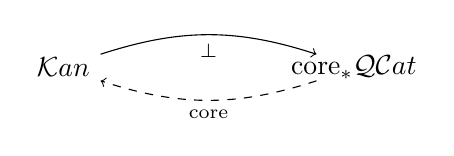
\begin{tikzpicture}[x=1.5em,y=1.2em]
  \node (Kan) at (0,0) {$\Kan$};
  \node (CQ)  at (7.0,0) {$\coreS\QCat$};
  \draw[->] (0.9,0.4) to[bend left=18] node[midway,below]{$\scriptstyle\perp$} (6.1,0.4);
  \draw[->,dashed] (6.1,-0.4) to[bend left=18] node[midway,below]{$\scriptstyle\mathrm{core}$} (0.9,-0.4);
\end{tikzpicture}
\end{center}
\end{lemma}

\begin{proof}
若 $K$ 与 $L$ 是\trKanComplex，则 $\Fun(K,L)$ 亦是。于是自然包含
$\Kan\hookrightarrow\QCat$ 经由 $(\infty,1)$-范畴核而分解。

右伴随 $\mathrm{core}\colon\coreS\QCat\to\QCat$ 在对象上按\cref{def:infinity-groupoid-core-quasi-category}的
构造作用。为定义其在诸\trFunctorSpace{}上的作用，我们必须对任何一对%
\trQuasiCategory{} $A$ 与 $B$ 提供一个典范映射
\begin{equation*}
\mathrm{core}(\Fun(A,B))\to\Fun(\mathrm{core}A,\mathrm{core}B)
\end{equation*}
由第 1 章中的\cref{cor:exponential-ideal}，$\Fun(A,B)\cong B^{A}$ 中的诸%
\trIsomorphism{}恰是那些单纯映射 $\alpha\colon A\times\Delta[1]\to B$：其
由 $A$ 的顶点 $a$ 标引的诸分量 $\alpha_{a}\colon\Delta[1]\to B$ 定义 $B$ 中
的\trIsomorphism。把这一观察与\cref{def:infinity-groupoid-core-quasi-category}相结合，我们看到
$\mathrm{core}(\Fun(A,B))$ 中的一个 $n$-单纯形是一个单纯映射
$\phi\colon A\times\Delta[n]\to B$，它具有如下性质：限制到 $A$ 的任何顶点与
$\Delta[n]$ 的任何边上时，所得 $B$ 中的边是一个\trIsomorphism。当 $A$ 限制
到其\trKanComplex{}核时，$\mathrm{core}A$ 的边也是\trIsomorphism。于是
$\phi\colon\mathrm{core}A\times\Delta[n]\to B$ 把定义域的每条边送到 $B$ 中
的一个\trIsomorphism，从而经由 $\mathrm{core}B\hookrightarrow B$ 分解，
因为这个包含在可逆的边上是满的。\footnote{在带标记单纯集的语言中，
$\mathrm{core}(\Fun(A,B))$ 中的一个映射是一个带标记映射
$A^{\sharp}\times\Delta[n]^{\sharp}\to B^{\flat}$。沿
$\mathrm{core}A^{\sharp}\hookrightarrow A^{\sharp}$ 限制后，定义域
$\mathrm{core}A^{\sharp}\times\Delta[n]^{\sharp}$ 是极大标记的，从而经由
极大标记的 $\mathrm{core}B^{\flat}\hookrightarrow B^{\flat}$ 分解（见 D.4
节）。}于是，这个 $n$-单纯形 $\phi$ 限制而定义一个 $n$-单纯形
$\phi\colon\mathrm{core}A\times\Delta[n]\to\mathrm{core}B$。这就定义了该
典范映射。

现在，对一个\trKanComplex{} $K$ 与一个\trQuasiCategory{} $A$，单纯自然%
\trIsomorphism
\begin{equation*}
\mathrm{core}(\Fun(K,A))\cong\Fun(K,\mathrm{core}A)
\end{equation*}
是易于验证的。顶点上的对应表达了非富集的\trAdjunction，而更高维单纯形上的
对应则循刚才讨论的理由以及\trIsomorphism{} $\mathrm{core}(K)\cong K$ 而得。
\end{proof}

\begin{corollary}\label{cor:core-of-equivalent-quasi-categories}
若 $A$ 与 $B$ 是\trEquivalence{}的\trQuasiCategory，则 $\mathrm{core}A$ 与
$\mathrm{core}B$ 是\trEquivalence{}的\trKanComplex。
\end{corollary}

\begin{proof}
诸\trQuasiCategory{}之间的一个\trEquivalence{}由一对 $0$-箭头连同可逆
$1$-箭头的一对所指定。如此，它包含于 $(\infty,1)$-范畴核
$\coreS\QCat\hookrightarrow\QCat$ 之中，并被\trSimplicialFunctor{}
$\mathrm{core}\colon\coreS\QCat\to\Kan$ 所保持。
\end{proof}

一个 $(\infty,1)$-\trCategory{}的一般\trInfinityCosmos{}中的一个%
\trInfinityCategory{}的核，可以按与\cref{def:opposite-infinity-category}类似的方式定义，但这个概念
还拥有一个到\trEquivalence{}为止的\trUniversalProperty，我们更愿意把它用作
定义。

\begin{definition}\label{def:infinity-groupoid-core-cosmos}
设 $\mathcal{K}$ 是一个 $(\infty,1)$-\trCategory{}的\trInfinityCosmos{}，
并设 $A$ 是 $\mathcal{K}$ 中的一个\trInfinityCategory。它的%
\textbf{\trInfinityGroupoidCore}是一个配有映射 $\iota\colon\mathrm{core}A\to A$
的\trInfinityCategory{} $\mathrm{core}A$，使得
\begin{itemize}
\item $\mathrm{core}A$ 是一个\trDiscrete{}\trInfinityCategory——意即对
  一切 $X$，$\Fun(X,\mathrm{core}A)$ 是一个\trKanComplex；%
  \footnote{原书此处印作「meaning that $\Fun(X,A)$ is a Kan complex for all
  $X$」。按本条首句所断言者乃 $\mathrm{core}A$ 之离散性，而\trDiscrete{}%
  \trInfinityCategory{}之定义（第 1 章中的\cref{def:discrete-infinity-categories}）
  正是「对一切 $X$，$\Fun(X,-)$ 皆为\trKanComplex」，故疑为
  $\Fun(X,\mathrm{core}A)$ 之误，此处径改。——译者注}
\item 若 $G$ 是一个\trDiscrete{}\trInfinityCategory，则 $\iota$ 定义一个%
  \trEquivalence
\begin{equation*}
\Fun(G,\mathrm{core}A)\xrightarrow{\ \iota\circ-\ }\mathrm{core}(\Fun(G,A))
\end{equation*}
\end{itemize}
\end{definition}

在实践中，一个 $(\infty,1)$-\trCategory{}的\trInfinityCosmos{}常常配有一个
显式的\trCoreFunctor{}；但与反者的情形一样，它也可以经由一个合适的%
\trChangeOfModel{}\trFunctor{}搬运核构造而定义：

\begin{proposition}\label{prop:core-quasi-pseudofunctor}
在一个 $(\infty,1)$-\trCategory{}的\trInfinityCosmos{} $\mathcal{K}$ 中，
任何一组对∞-\trInfinityGroupoidCore{}的选取都装配成一个拟伪\trFunctor{}
$\mathrm{core}\colon\coreS\mathcal{K}\to\Disc(\mathcal{K})$。特别地，对任意%
\trInfinityCategory{} $A,B\in\mathcal{K}$，存在一个映射
$\mathrm{core}(\Fun(A,B))\to\Fun(\mathrm{core}A,\mathrm{core}B)$，它在 $A$
与 $B$ 上（作为 $\coreS\mathcal{K}$ 的对象）都是拟伪自然的。
\end{proposition}

\begin{proof}
该拟伪\trFunctor{}定义为某个之字形链的复合，其中逆向的映射是一个%
\trCosmologicalBiequivalence，依据是推论 10.3.7：
\begin{center}
\begin{tikzpicture}[x=1.7em,y=1.5em]
  \node (tl) at (0,1.6) {$\coreS\mathcal{K}$};
  \node (tr) at (6.4,1.6) {$\Disc(\mathcal{K})$};
  \draw[->] (1.1,1.6) -- ++(0.60,0.07) -- ++(0.60,-0.14) -- ++(0.60,0.14)
    -- ++(0.60,-0.14) -- ++(0.60,0.14) -- ++(0.60,-0.14) -- ++(0.60,0.07);
  \node at (3.2,2.0) {$\scriptstyle\mathrm{core}(-)$};
  \draw[right hook->] (0,1.1) -- (0,0.45);
  \node at (-0.9,0.78) {$\scriptstyle(-)_{0}$};
  \node at (3.2,0.78) {$\scriptstyle\cong$};
  \draw[right hook->] (6.4,1.1) -- (6.4,0.45);
  \node at (7.3,0.78) {$\scriptstyle(-)_{0}$};
  \node (bl) at (0,0) {$\coreS\QCat$};
  \node (br) at (6.4,0) {$\Kan\cong\Disc(\QCat)$};
  \draw[->] (1.5,0) -- node[above]{$\scriptstyle\sim$}
    node[below]{$\scriptstyle\mathrm{core}(-)$} (3.9,0);
\end{tikzpicture}
\end{center}
我们把「$\mathcal{K}\rightsquigarrow\mathcal{L}$ 下降为一个单纯富集的%
\trBiequivalence{} $\coreS\mathcal{K}\rightsquigarrow\coreS\mathcal{L}$」的验证
留给\cref{ex:core-functor-biequivalence}。由命题 10.4.16，%
宇宙论\trBiequivalence{} $(-)_{0}\colon\Disc(\mathcal{K})\Rightarrow\Kan$
的逆定义一个拟伪\trFunctor{}与\trBiequivalence{}
$\Kan\rightsquigarrow\Disc(\mathcal{K})$，后者与单纯\trFunctor{}
$\mathrm{core}((-)_{0})\colon\coreS\mathcal{K}\to\Kan$ 相复合而定义拟伪%
\trFunctor{} $\mathrm{core}\colon\coreS\mathcal{K}\to\Disc(\mathcal{K})$。
由引理 10.4.12，这个拟伪\trFunctor{}在各 hom 上的作用定义一个拟伪自然变换。

尚待验证的只是：该拟伪\trFunctor{}在对象上的作用满足\cref{def:infinity-groupoid-core-cosmos}
的诸条件。由构造，对任何 $A\in\mathcal{K}$，$\mathrm{core}A$ 是一个%
\trDiscrete{}\trInfinityCategory。映射 $\iota\colon\mathrm{core}A\to A$
定义为把「\trQuasiCategory{}的\trKanComplex{}核的相应包含」与「底%
\trQuasiCategory{}\trFunctor{}及其拟伪\trFunctor{}性的逆」作须化：
\begin{equation*}
\coreS\mathcal{K}\;\xrightarrow[\ \sim\ ]{(-)_{0}}\;\coreS\QCat\;\;
\overset{\mathrm{core}}{\underset{\hookrightarrow}{\rightleftarrows}}\;\;
\coreS\QCat\;\overset{(-)_{0}^{-1}}{\rightsquigarrow}\;\coreS\mathcal{K}
\end{equation*}
现在，若 $G$ 是一个\trDiscrete{}\trInfinityCategory，则
$G_{0}=\Fun(1,G)$ 是一个\trKanComplex，于是由\cref{lem:kan-inclusion-factors-through-core}，
$\iota_{A_{0}}\circ-\colon\Fun(G_{0},\mathrm{core}(A_{0}))\rightsquigarrow\mathrm{core}(\Fun(G_{0},A_{0}))$
是一个\trEquivalence。由构造，$\mathrm{core}A$ 定义成使得
$(\mathrm{core}A)_{0}\cong\mathrm{core}(A_{0})$。注意：由于
$(-)_{0}\colon\mathcal{K}\Rightarrow\QCat$ 是一个\trBiequivalence，这表明：
一个 $(\infty,1)$-\trCategory{}的\trInfinityCosmos{}中的一个%
\trInfinityCategory{}的核在\trEquivalence{}意义下是良定义的。由于单纯%
\trFunctor{} $(-)_{0}\colon\coreS\mathcal{K}\to\coreS\QCat$ 在各 hom 上是%
\trEquivalence，由与 $\iota_{A}$ 作后复合所定义的\trFunctor{}等价于这个%
\trFunctor
\begin{center}
\begin{tikzpicture}[x=1.6em,y=1.5em]
  \node (tl) at (0,1.6) {$\Fun(G,\mathrm{core}A)$};
  \node (tr) at (7.0,1.6) {$\mathrm{core}(\Fun(G,A))$};
  \draw[->] (tl) -- node[above]{$\scriptstyle\iota_{A}\circ-$} (tr);
  \draw[right hook->] (0,1.1) -- (0,0.45);
  \node at (-0.9,0.78) {$\scriptstyle(-)_{0}$};
  \node at (3.5,0.78) {$\scriptstyle\cong$};
  \draw[right hook->] (7.0,1.1) -- (7.0,0.45);
  \node at (7.9,0.78) {$\scriptstyle(-)_{0}$};
  \node (bl) at (0,0) {$\Fun(G_{0},\mathrm{core}A_{0})$};
  \node (br) at (7.0,0) {$\mathrm{core}(\Fun(G_{0},A_{0}))$};
  \draw[->] (bl) -- node[above]{$\scriptstyle\sim$}
    node[below]{$\scriptstyle\iota_{A_{0}}\circ-$} (br);
\end{tikzpicture}
\end{center}
于是，与 $\iota_{A}$ 的后复合诱导所需的\trEquivalence{}
$\Fun(G,\mathrm{core}A)\cong\mathrm{core}(\Fun(G,A))$，证明完成。
\end{proof}

\subsection*{练习}

\begin{exercise}\label{ex:homotopy-category-of-opposite}
证明：一个\trInfinityCategory{} $A$ 之反者的\trHomotopyCategory\trEquivalence{}%
于 $A$ 的\trHomotopyCategory{}之反者。
\end{exercise}

\begin{exercise}\label{ex:opposite-of-equivalence}
证明：诸\trInfinityCategory{}之间的一个\trFunctor{}是一个\trEquivalence，
当且仅当其反\trFunctor{}是一个\trEquivalence。
\end{exercise}

\begin{exercise}\label{ex:marked-enrichment-core}
在 D.4 节与 D.5 节的协助下：
\begin{enumerate}[label=(\roman*)]
\item 重新定义第 1 章中的\cref{def:infinity-cosmos}的\trInfinityCosmos{}%
  概念，使之成为一个富集于带标记单纯集之上的\trCategory{}，其诸%
  \trFunctorSpace{}为自然标记的\trQuasiCategory。
\item 描述带这种富集的\trInfinityCosmos{}中、一个自然标记的%
  \trQuasiCategory{}的\trInfinityGroupoidCore{}以及一个\trInfinityCosmos{}%
  的 $(\infty,1)$-范畴核的构造。
\item 证明 $(\infty,1)$-范畴核与单纯集作余张量，尽管这些\trCotensor{}并不
  被包含 $\coreS\mathcal{K}\hookrightarrow\mathcal{K}$ 所保持。
\item 证明一个\trInfinityCosmos{}的 $(\infty,1)$-核是新意义下的一个%
  \trInfinityCosmos{}，尽管\trFunctor{}
  $\coreS\mathcal{K}\hookrightarrow\mathcal{K}$ 仍不是宇宙论的。
\end{enumerate}
\end{exercise}

\begin{exercise}\label{ex:core-functor-biequivalence}
设 $F\colon\mathcal{K}\to\mathcal{L}$ 是一个\trCosmologicalFunctor。证明：
$F$ 诱导一个单纯\trFunctor{} $F\colon\coreS\mathcal{K}\to\coreS\mathcal{L}$，
并且若原来的\trFunctor{}是一个\trBiequivalence，则它也是一个\trBiequivalence。
\end{exercise}

\begin{exercise}\label{ex:adjunction-restricts-adjoint-equivalence}
\begin{enumerate}[label=(\roman*)]
\item 证明：诸\trQuasiCategory{}之间的任何\trAdjunction
\begin{center}
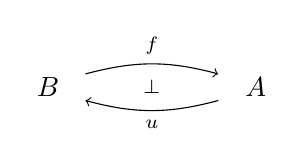
\begin{tikzpicture}[x=1.5em,y=1.2em]
  \node (B) at (0,0) {$B$};
  \node (A) at (5.0,0) {$A$};
  \draw[->] (0.9,0.4) to[bend left=15] node[above,pos=0.5]{$\scriptstyle f$} (4.1,0.4);
  \node at (2.5,0) {$\scriptstyle\perp$};
  \draw[->] (4.1,-0.4) to[bend left=15] node[below,pos=0.5]{$\scriptstyle u$} (0.9,-0.4);
\end{tikzpicture}
\end{center}
都限制而定义一个介于诸全子拟范畴之间的伴随\trEquivalence——这些全子拟范畴
由那些使单位与余单位分量（各自地）可逆的\trElement{} $b\colon 1\to B$ 与
$a\colon 1\to A$ 张成。
\item 陈述并证明一个关于伴随\trEquivalence{}的类似结果，其中的伴随%
\trEquivalence{}由任意一个 $(\infty,1)$-\trCategory{}的\trInfinityCosmos{}%
中的诸\trAdjunction{}导出。
\end{enumerate}
\end{exercise}

